%!TEX root = ../Demo.tex
\chapter{类图}

\begin{figure}[!htbp]
    \centering
        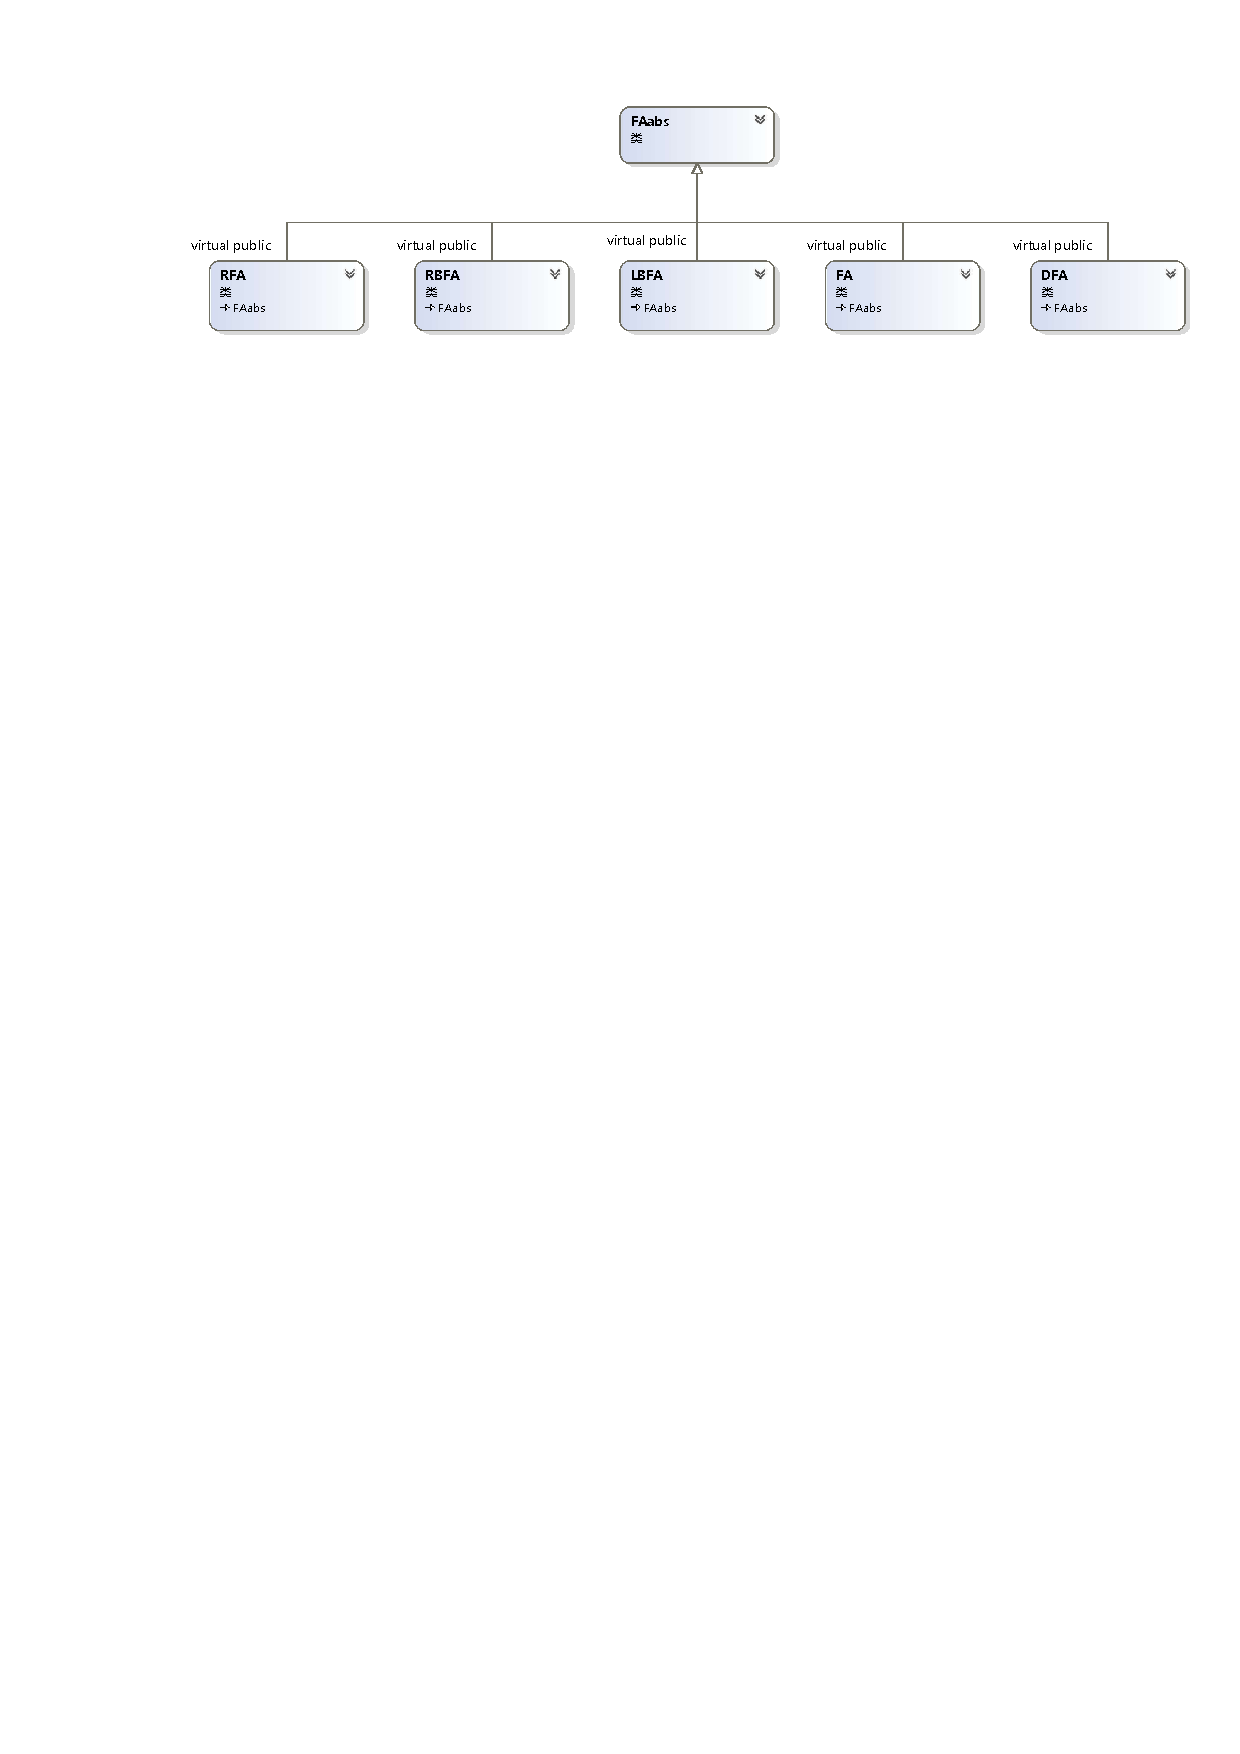
\includegraphics[width=0.98\textwidth]{classdiagram/FAabs.pdf}
    \caption{类 FAabs 及其派生类}
    \label{fig:class-faabs}
\end{figure}

箭头 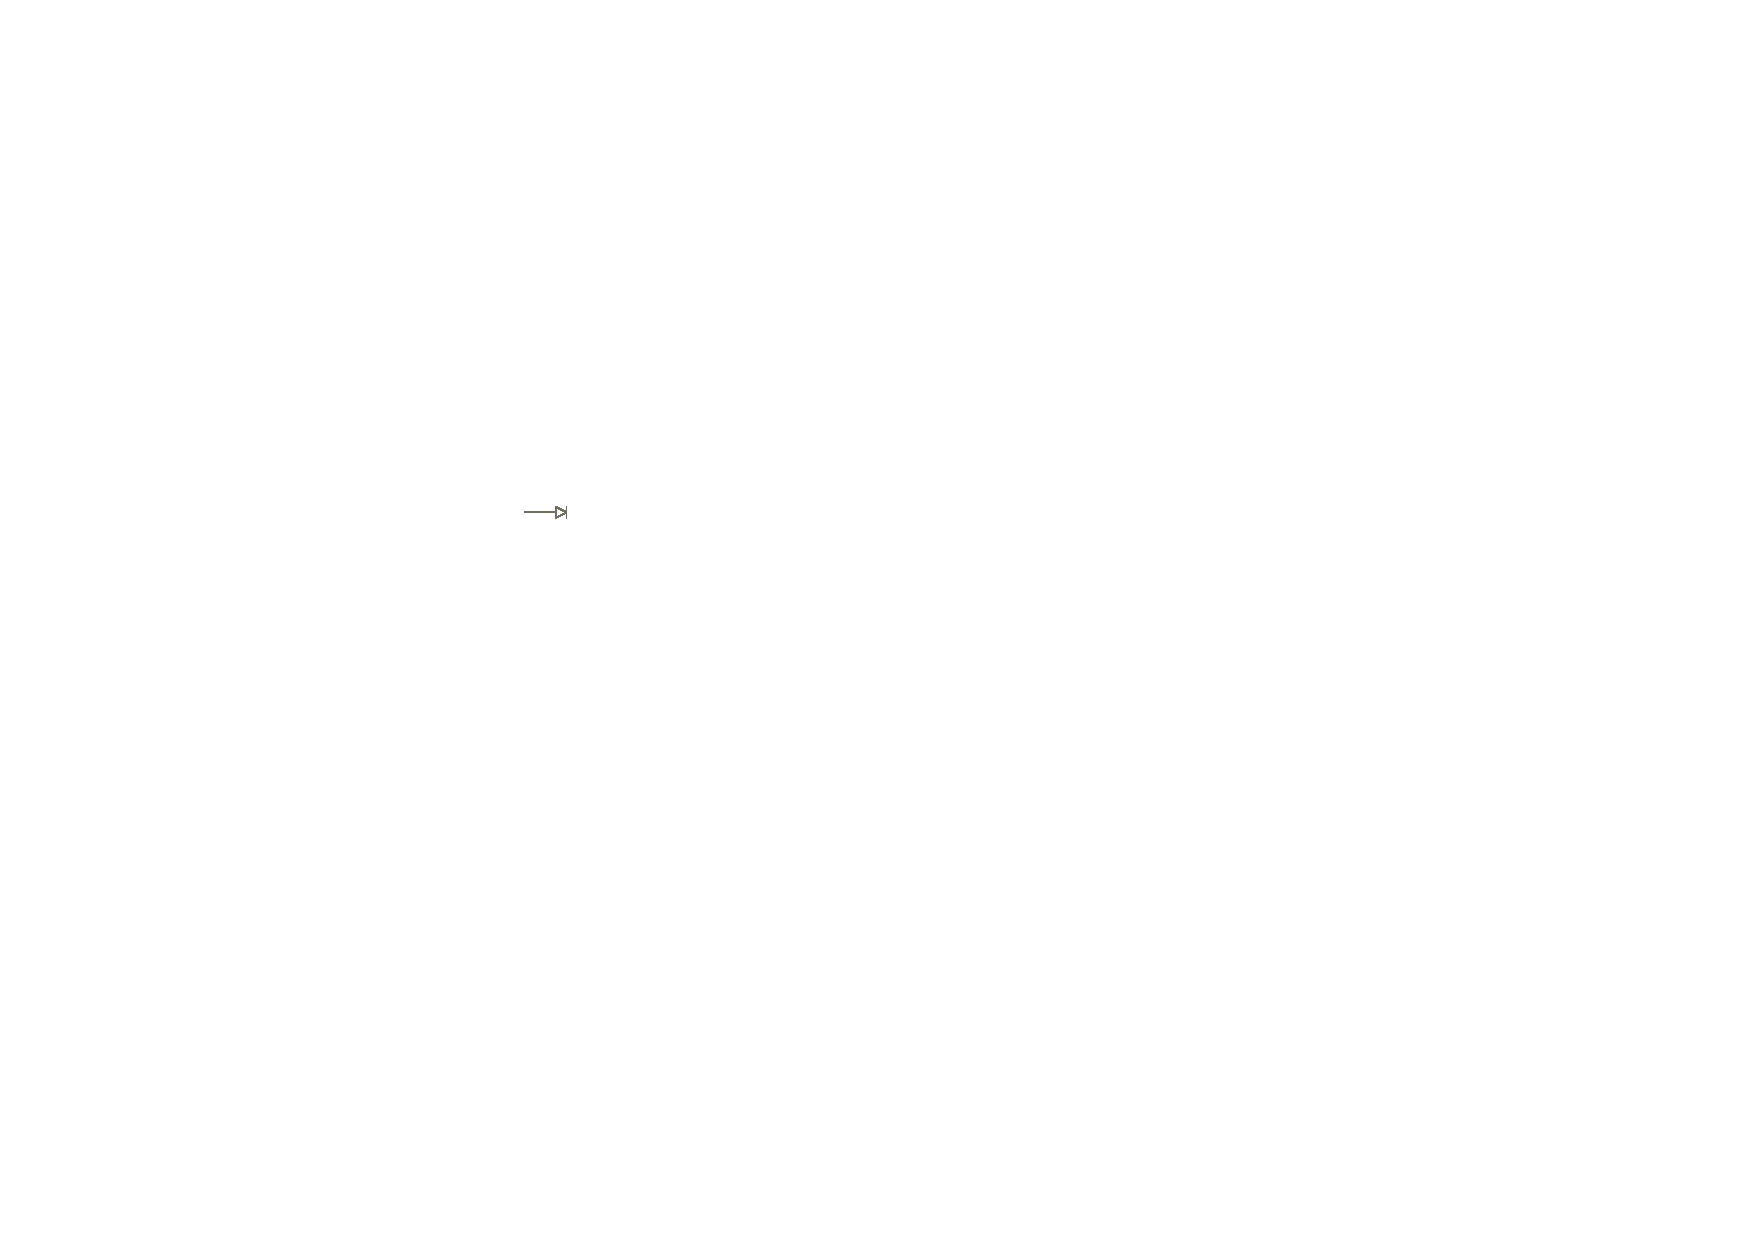
\includegraphics{jicheng.pdf} 由派生类指向基类。箭头 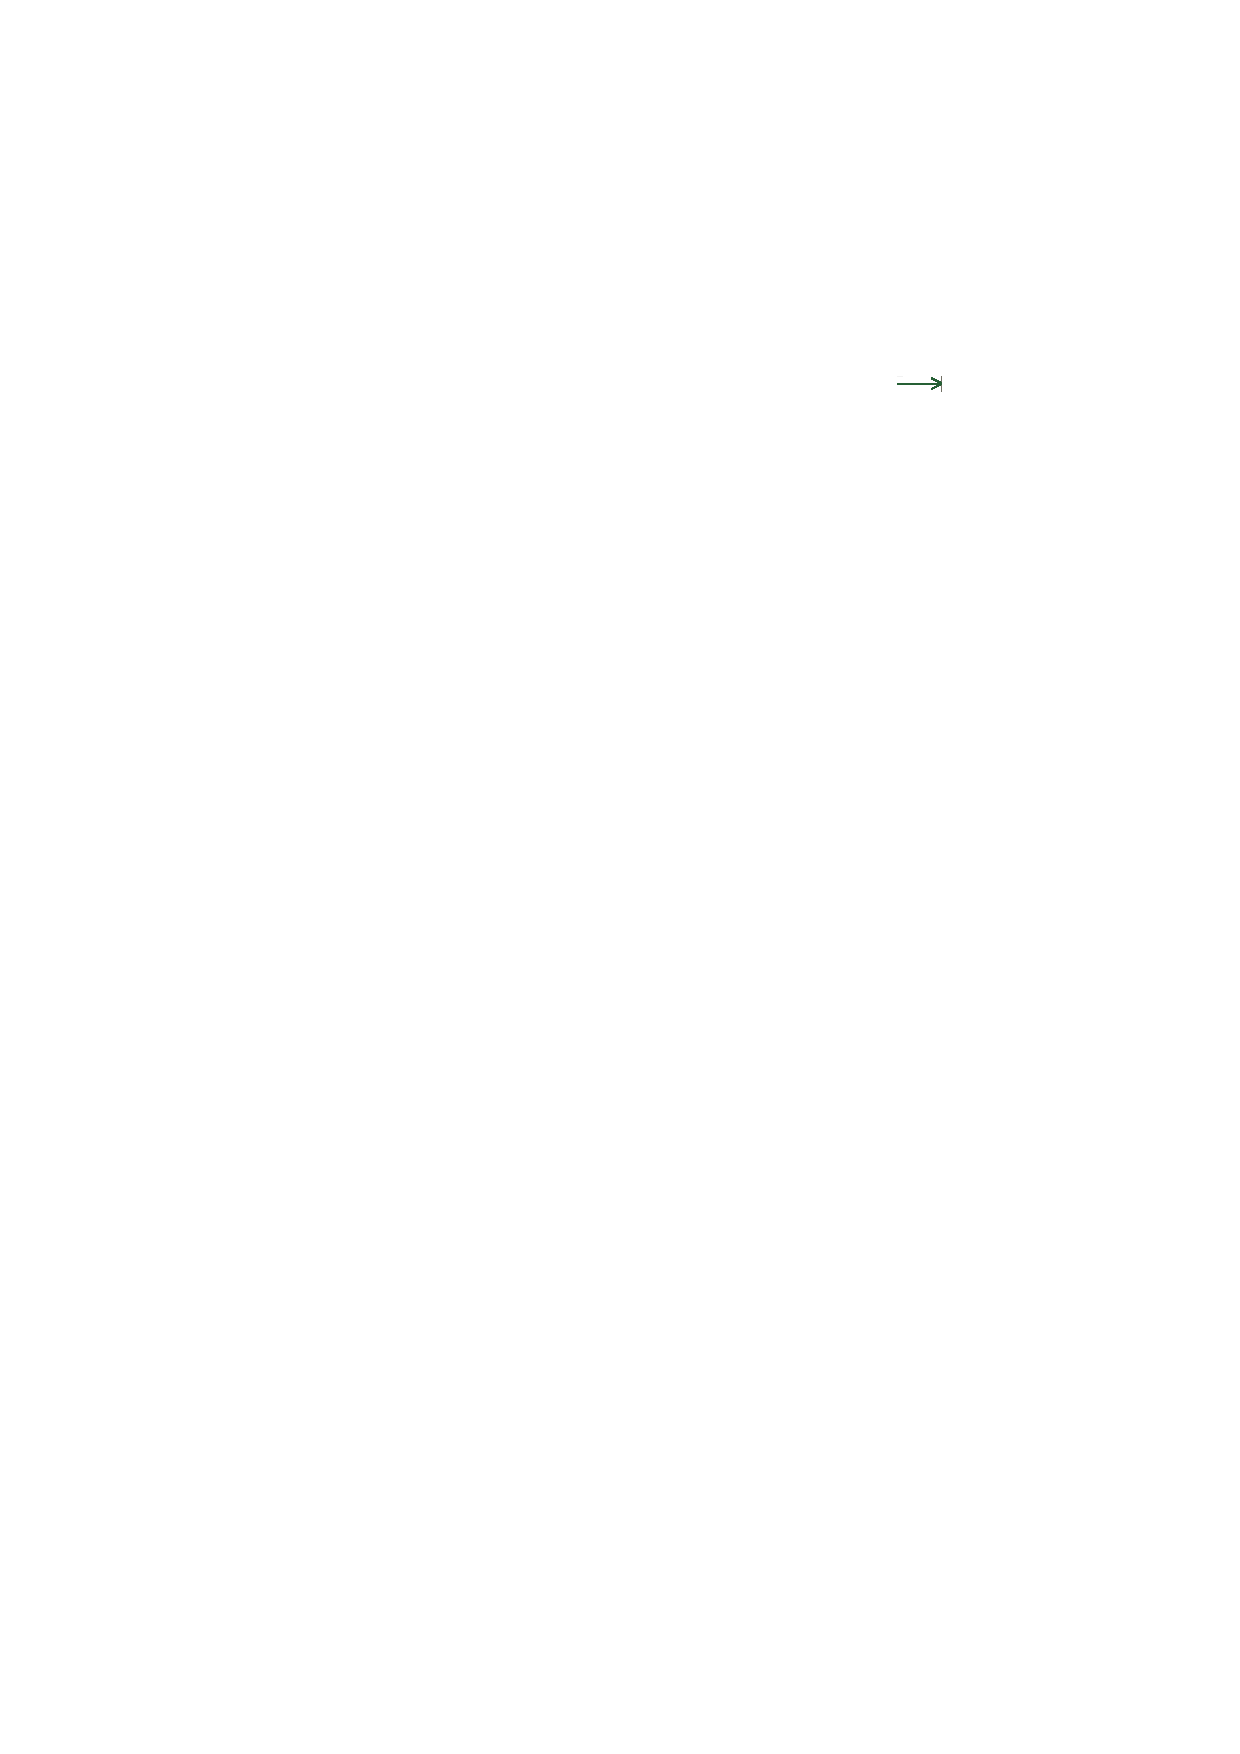
\includegraphics{chengyuan.pdf} 从一个类指向其成员变量的类型,箭头上方标注了该成员变量的名称。

% \begin{figure}[!htbp]
%     \centering
%         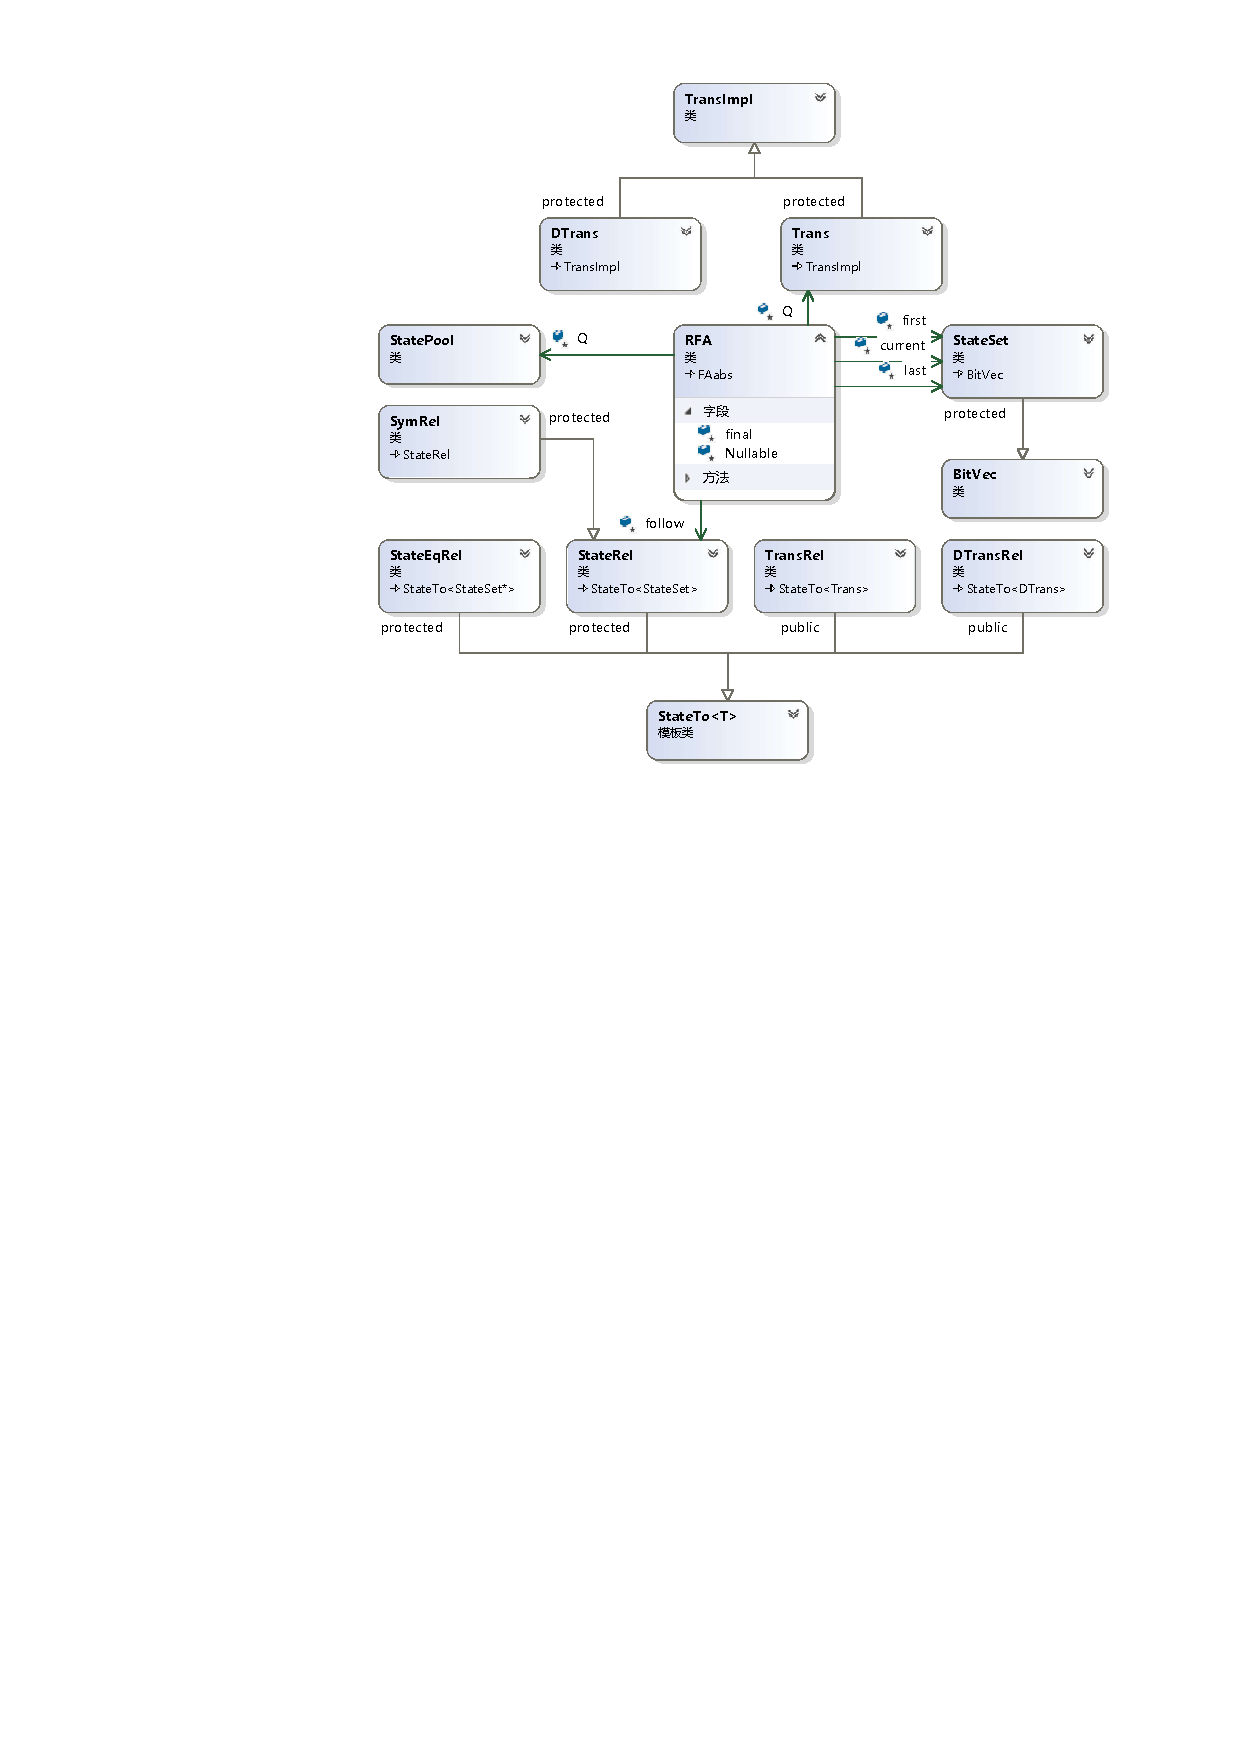
\includegraphics[width=0.98\textwidth]{classdiagram/RFA.pdf}
%     \caption{类 RFA 与其成员类及成员类的基类}
%     \label{fig:class-rfa}
% \end{figure}



% \begin{figure}[!htbp]
%     \centering
%         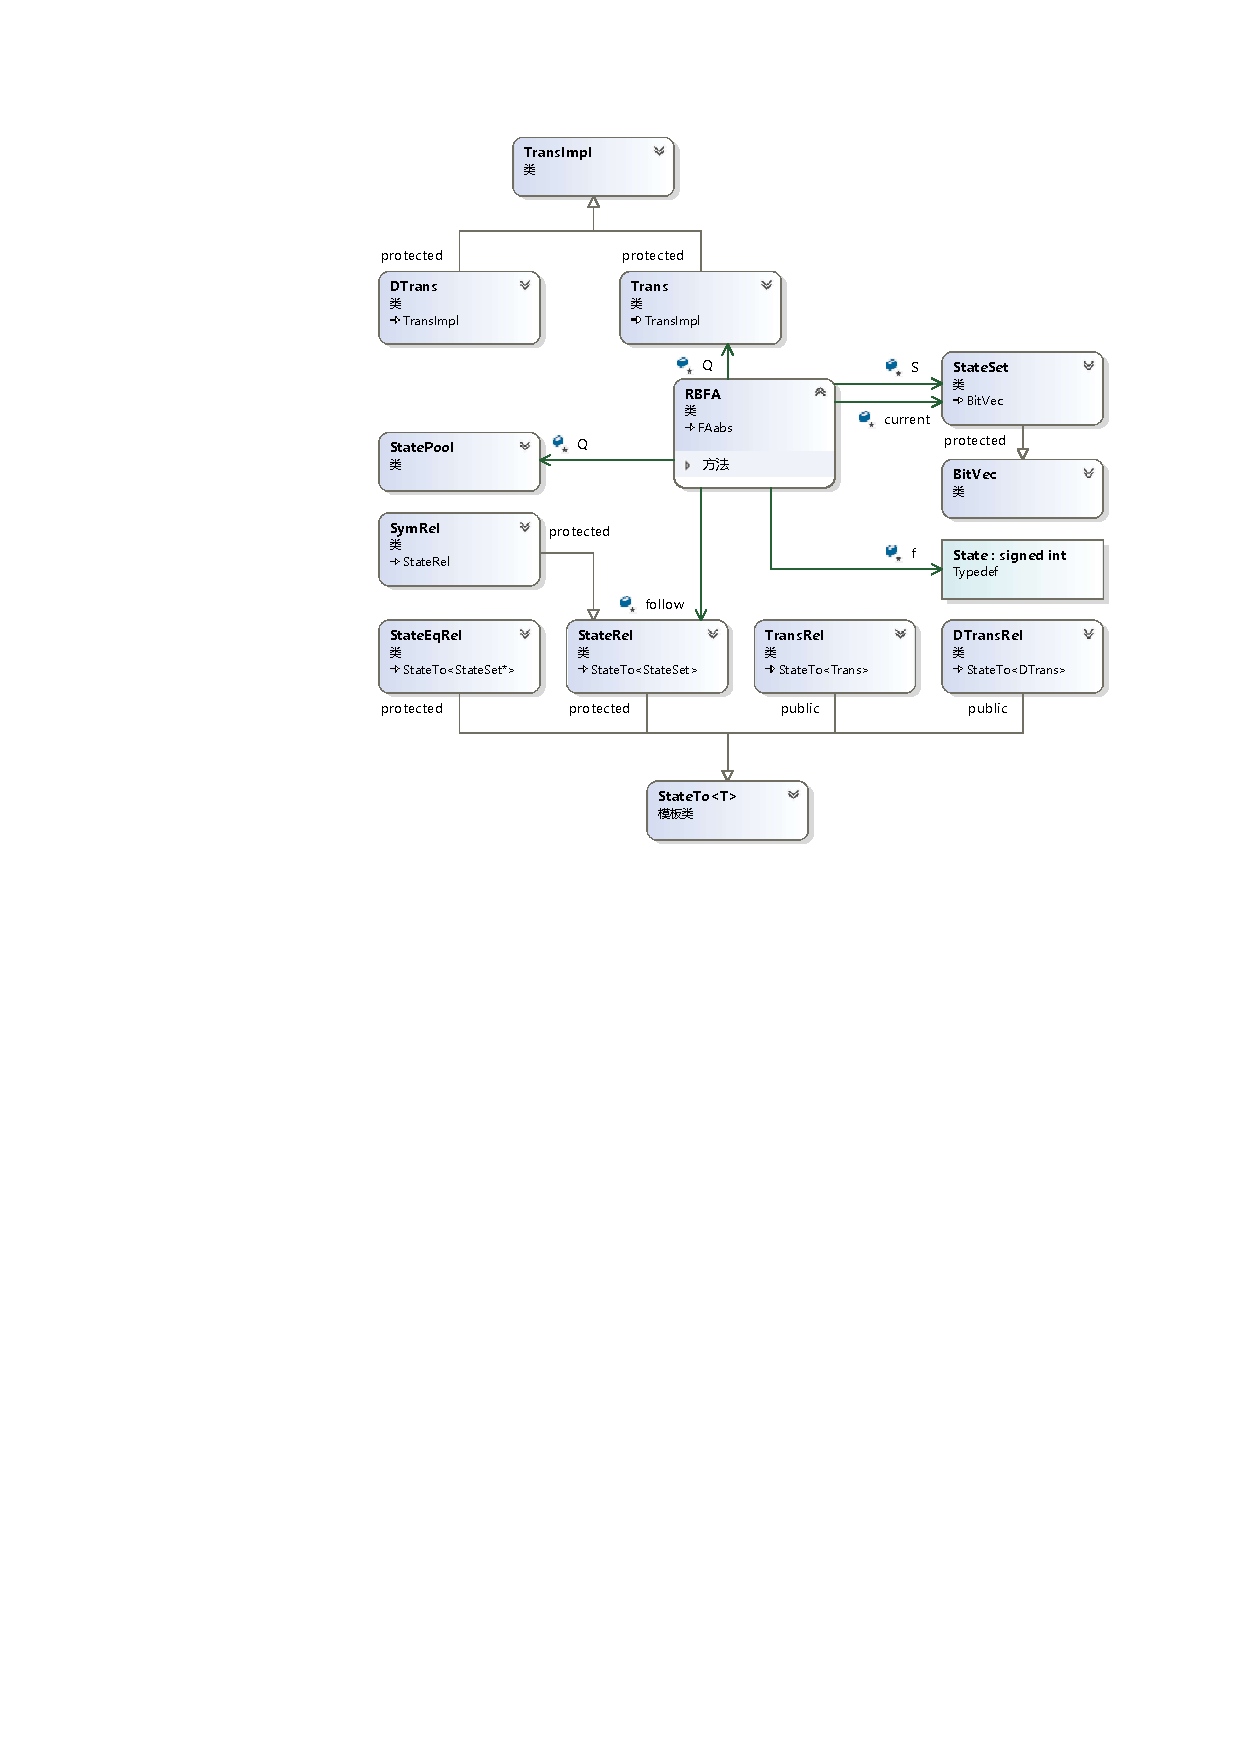
\includegraphics[width=0.98\textwidth]{classdiagram/RBFA.pdf}
%     \caption{类 RBFA 与其成员类及成员类的基类}
%     \label{fig:class-rbfa}
% \end{figure}

% \begin{figure}[!htbp]
%     \centering
%         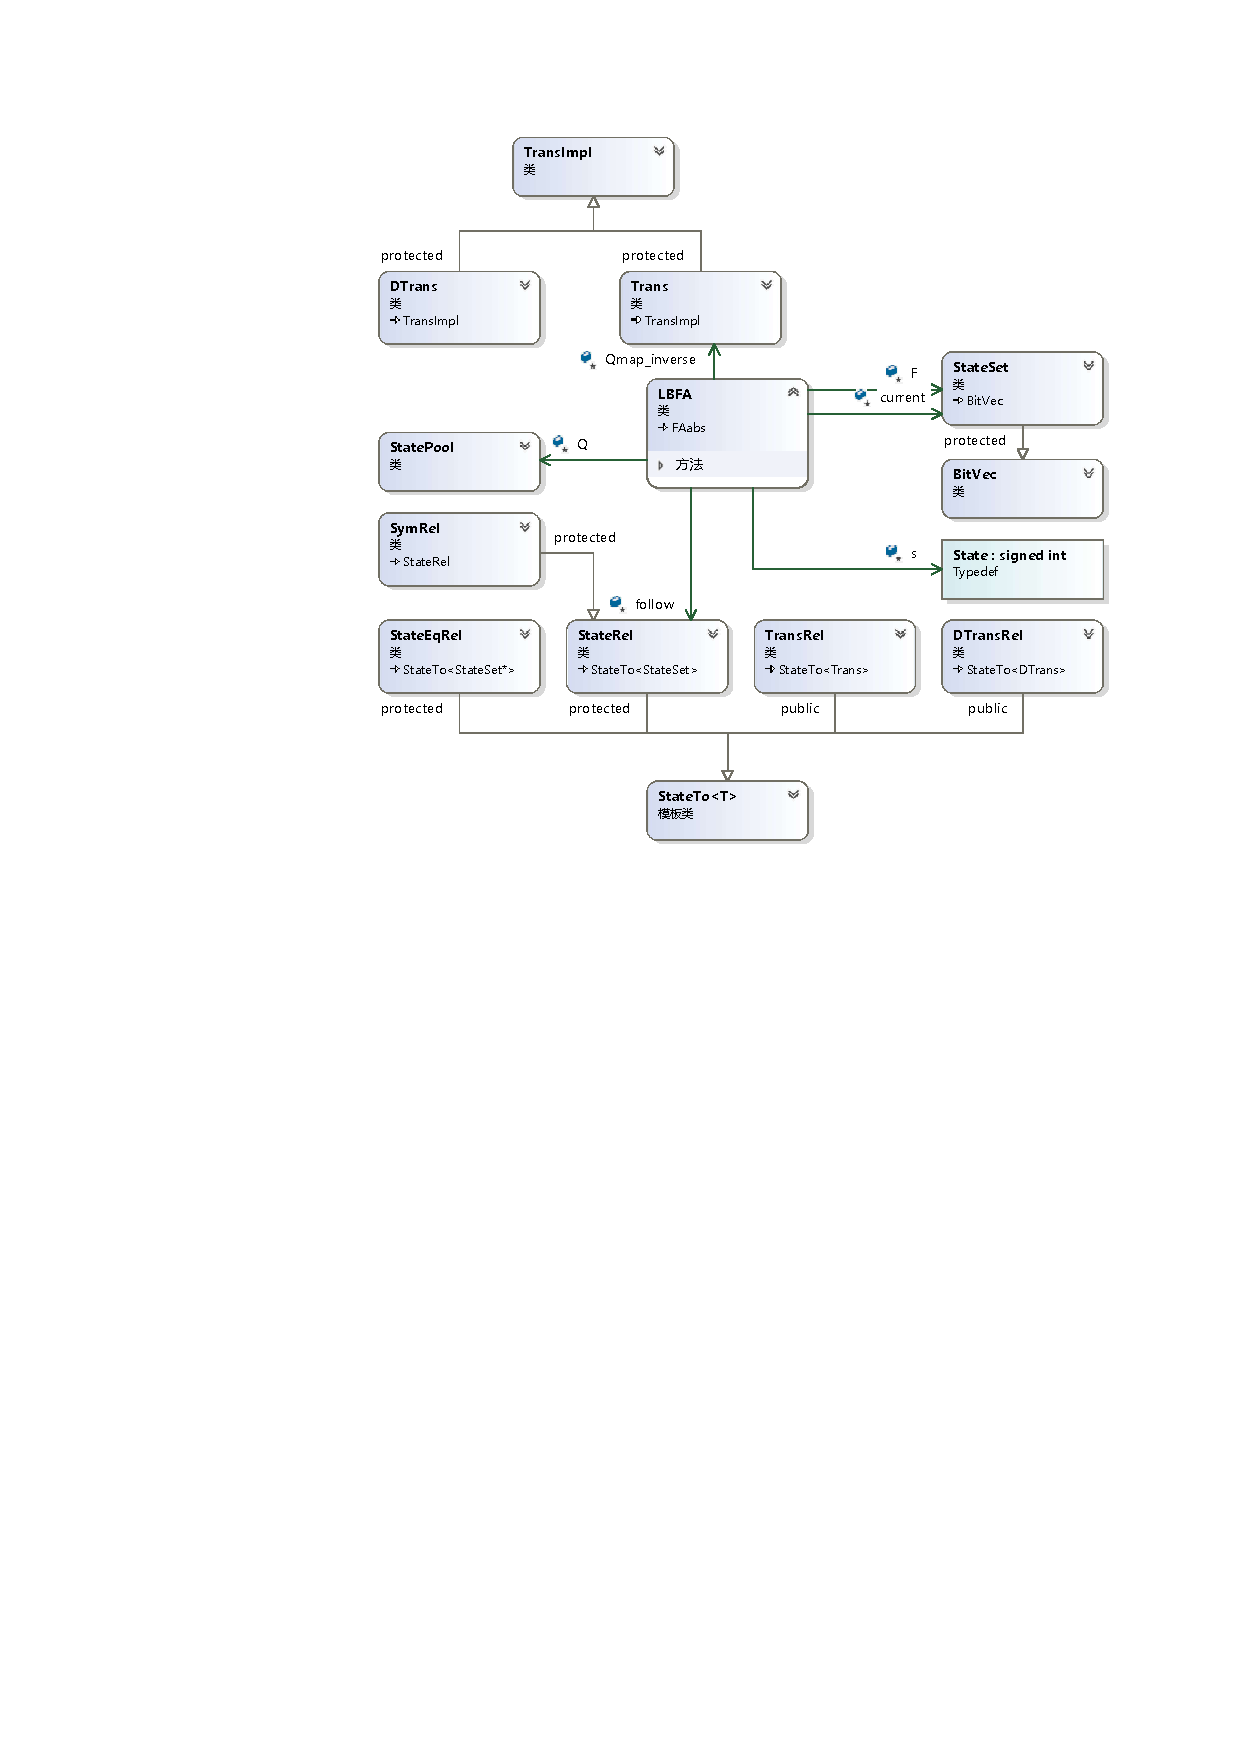
\includegraphics[width=0.98\textwidth]{classdiagram/LBFA.pdf}
%     \caption{类 LBFA 与其成员类及成员类的基类}
%     \label{fig:class-lbfa}
% \end{figure}

% \begin{figure}[!htbp]
%     \centering
%         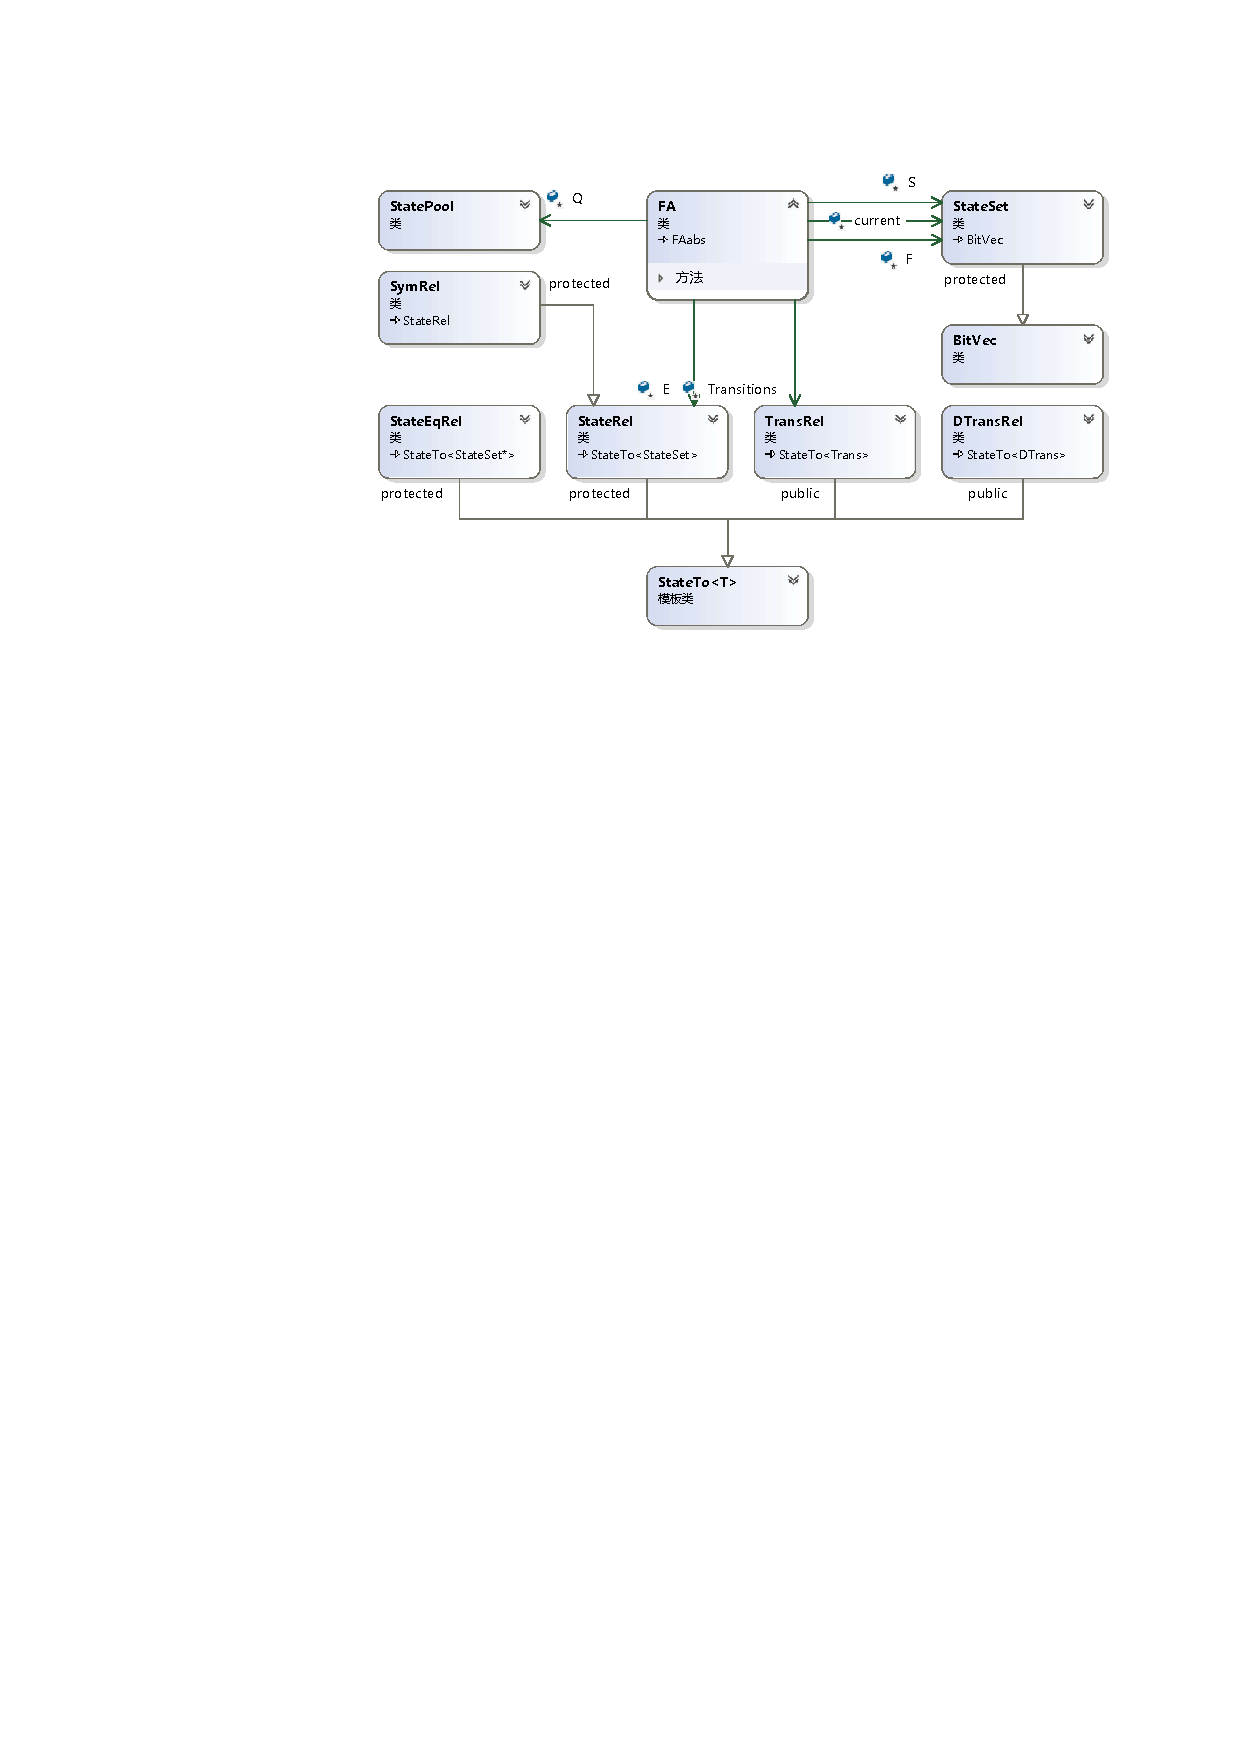
\includegraphics[width=0.98\textwidth]{classdiagram/FA.pdf}
%     \caption{类 FA 与其成员类及成员类的基类}
%     \label{fig:class-fa}
% \end{figure}

\begin{figure}[!htbp]
    \centering
        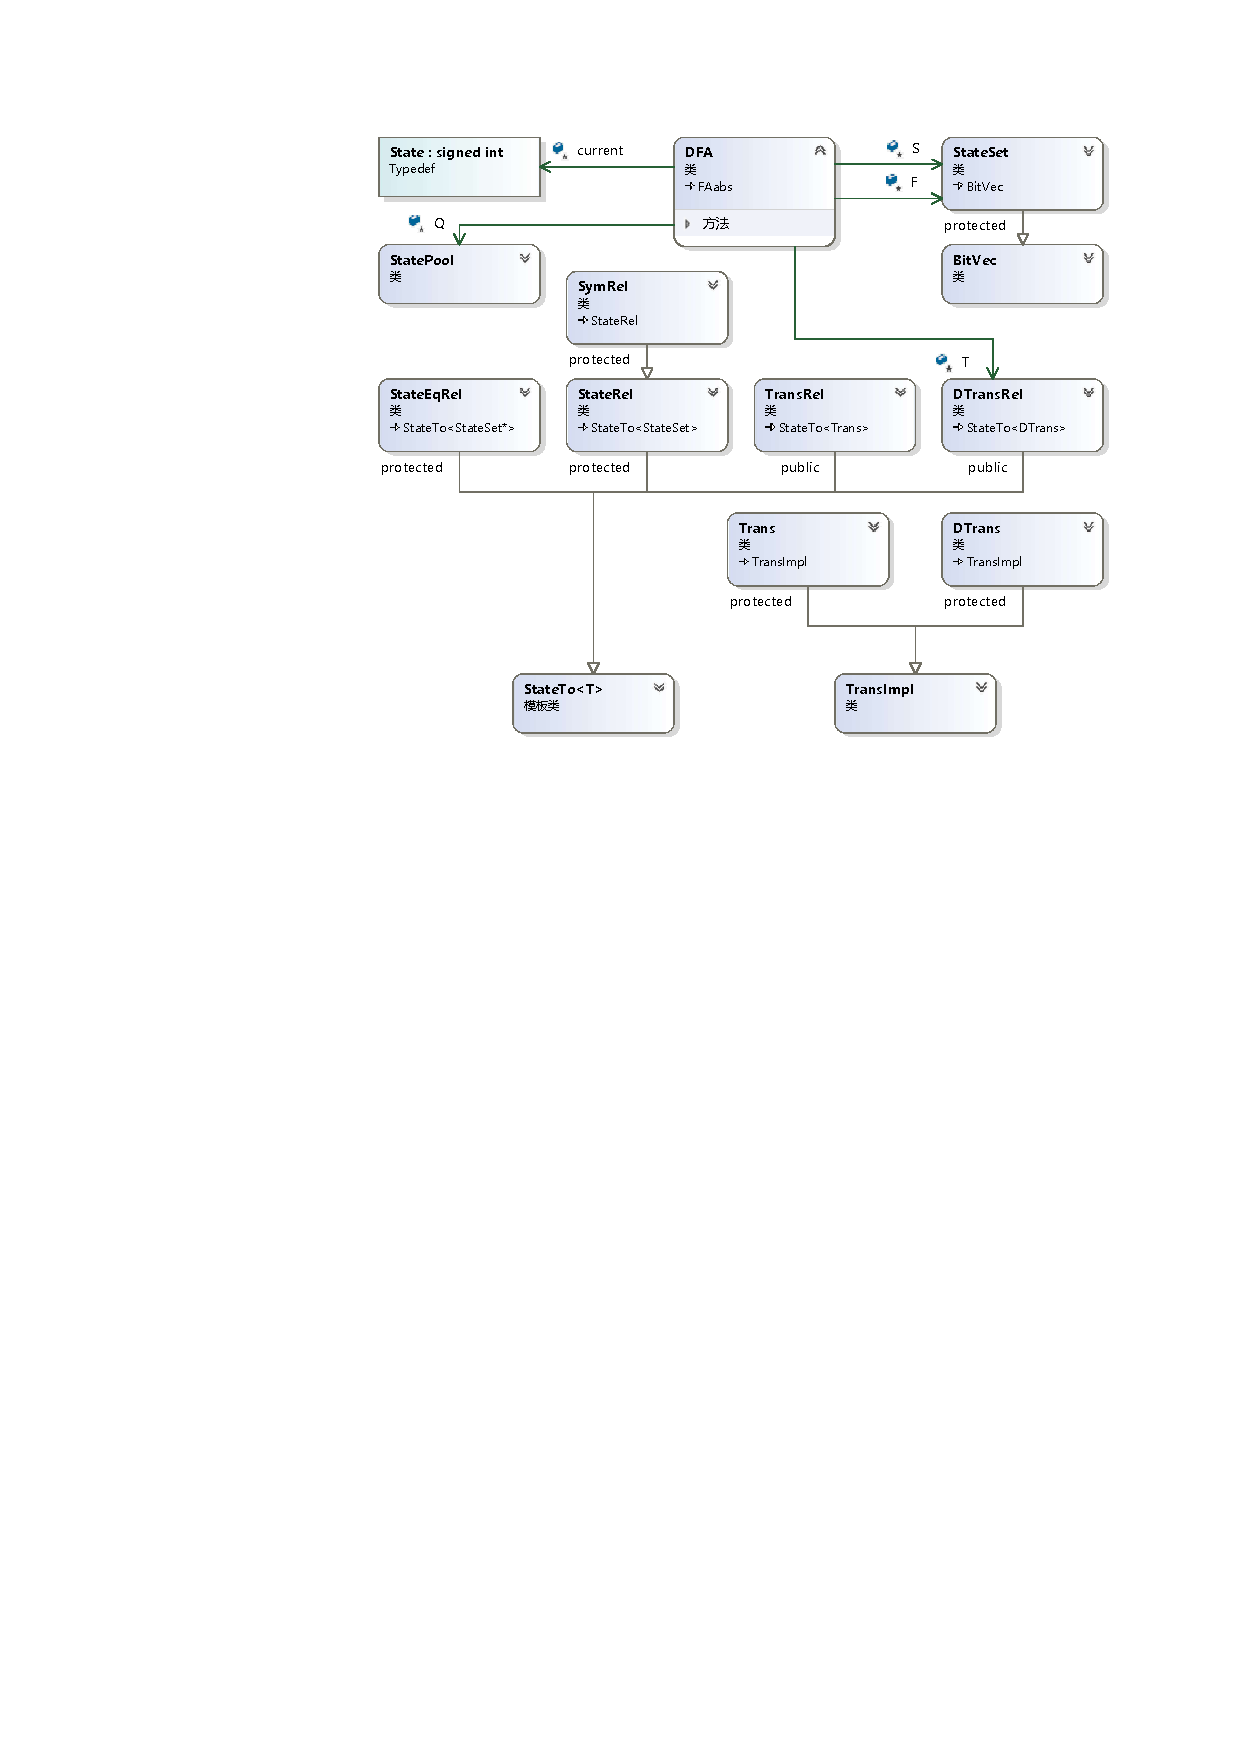
\includegraphics[width=0.98\textwidth]{classdiagram/DFA.pdf}
    \caption{类 DFA 与其成员类及成员类的基类}
    \label{fig:class-dfa}
\end{figure}

\begin{figure}[!htbp]
    \centering
        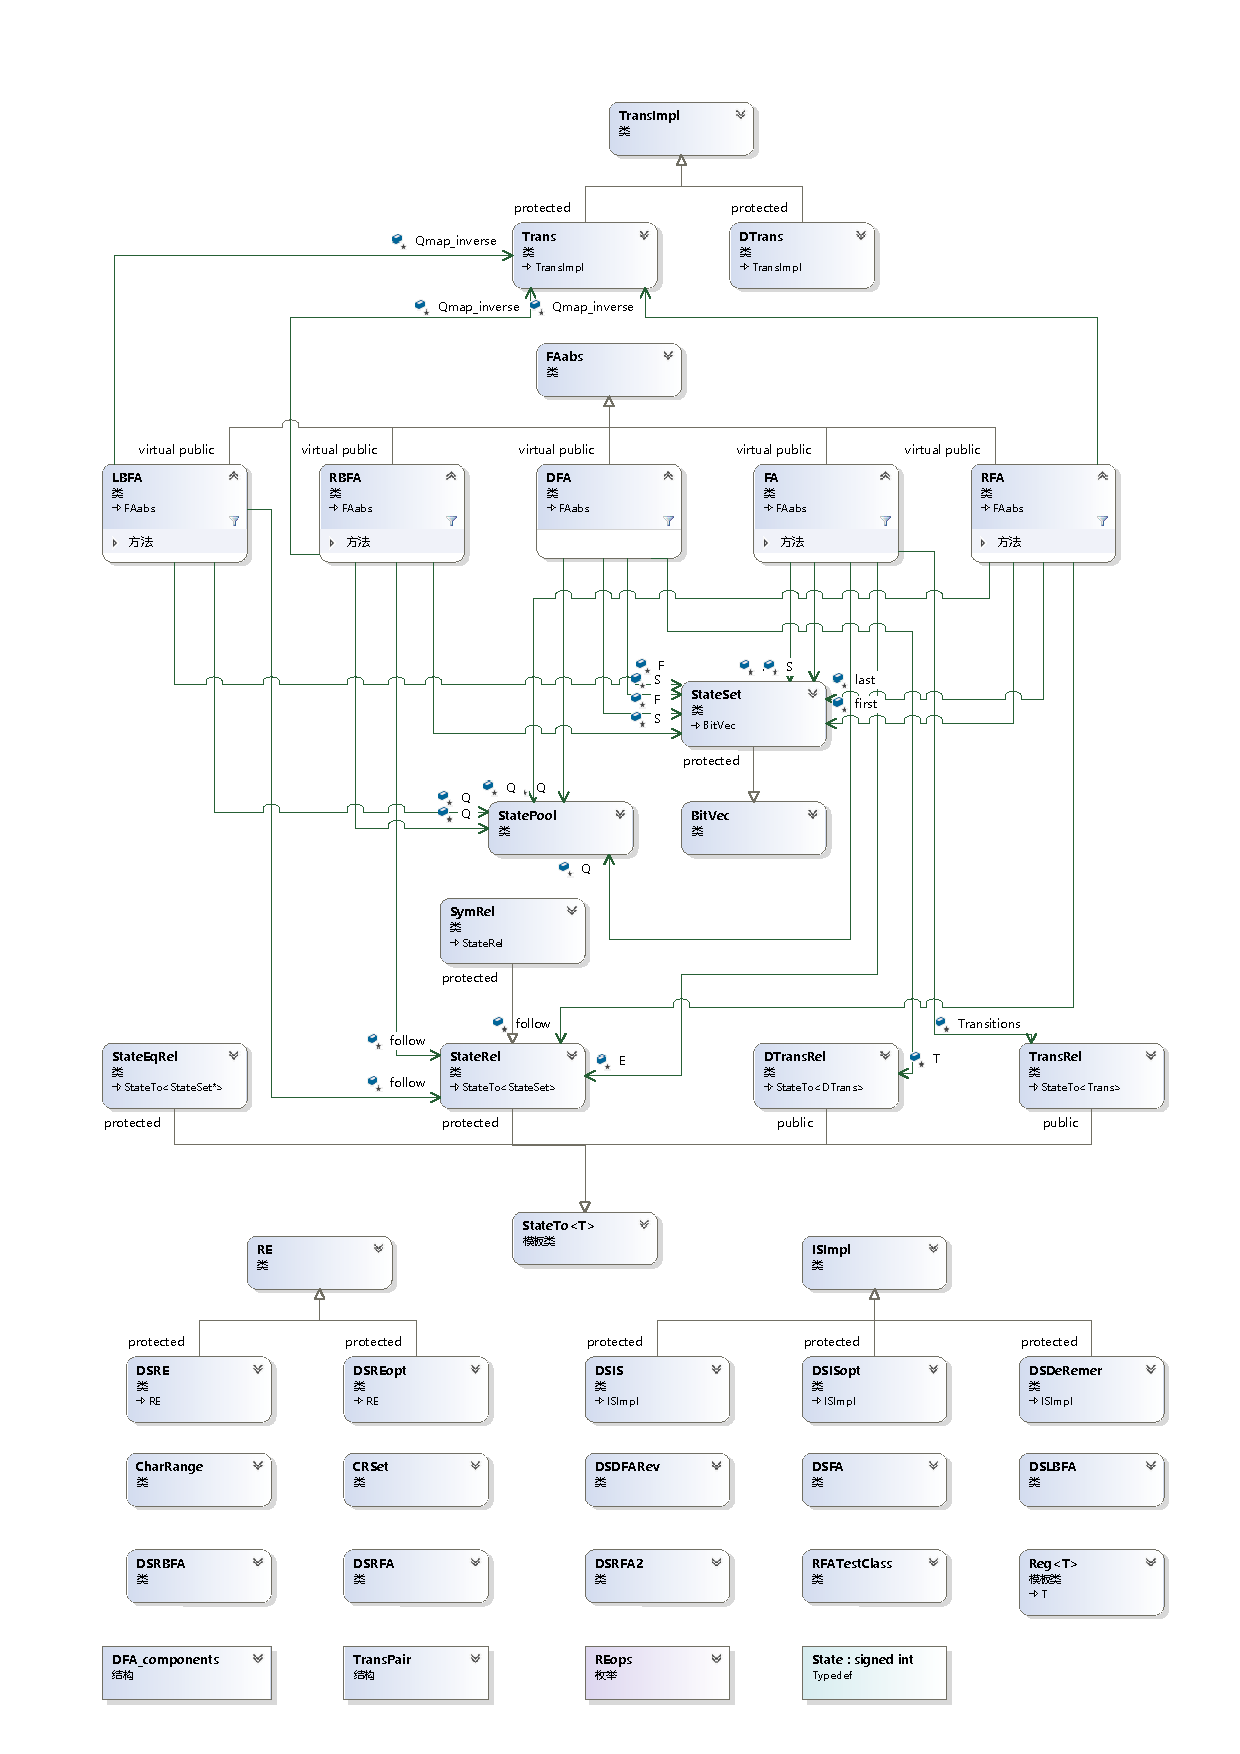
\includegraphics[width=0.98\textwidth]{classdiagram/FIRE_engine.pdf}
    \caption{FIRE engine 的构成}
    \label{fig:FIRE-engine}
\end{figure}